\documentclass[11pt]{book}
\usepackage{fontspec}
\setmainfont{TeX Gyre Pagella}
\usepackage[margin=1in]{geometry}
\usepackage{xcolor}
\usepackage{tikz}
\usetikzlibrary{arrows.meta,shapes.geometric,shapes.misc}
\usepackage{amssymb}
\usepackage{enumitem}
\usepackage{titlesec}

\titleformat{\chapter}[display]{\bfseries\Large}{Sproll 09}{0.5em}{\Huge}
\titleformat{\section}{\bfseries\large}{\thesection}{0.6em}{}

\newenvironment{algorithmproc}[1]{\vspace{0.6em}\noindent\rule{\linewidth}{0.6pt}\\[0.2em]\textbf{How to Tell: #1}\\[0.3em]}{\\[0.2em]\noindent\rule{\linewidth}{0.6pt}\vspace{0.6em}}
\newenvironment{practicenow}{\vspace{0.6em}\noindent\rule{\linewidth}{0.6pt}\\[0.2em]\textbf{Practice Now}\\[0.3em]}{\\[0.2em]\noindent\rule{\linewidth}{0.6pt}\vspace{0.6em}}
\newenvironment{exercisebox}[1]{\vspace{0.8em}\noindent\rule{\linewidth}{0.6pt}\\[0.2em]\textbf{Exercises: #1}\\[0.3em]\begin{enumerate}[label=\arabic*., itemsep=0.4em]}{\end{enumerate}\noindent\rule{\linewidth}{0.6pt}\vspace{0.6em}}
\newenvironment{trythis}{\vspace{0.6em}\noindent\rule{\linewidth}{0.6pt}\\[0.2em]\textbf{Try This}\\[0.3em]}{\\[0.2em]\noindent\rule{\linewidth}{0.6pt}\vspace{0.6em}}
\newenvironment{summarybox}{\vspace{0.6em}\noindent\rule{\linewidth}{0.6pt}\\[0.2em]\textbf{What We Learned}\\[0.3em]}{\\[0.2em]\noindent\rule{\linewidth}{0.6pt}\vspace{0.6em}}

\begin{document}
\begin{titlepage}
\centering
\vspace*{1.4in}
{\Huge \textbf{SPROLL 09}}\\[0.5in]
{\huge Parts With a Past}\\[0.8in]

\begin{tikzpicture}
\draw[line width=1pt, gray!45] (-0.3,0) circle (0.5in);
\filldraw[fill=black] (0,0) circle (0.22in);
\end{tikzpicture}\\[0.8in]
{\Large The Sproll Curriculum}\\[0.2in]
{\large Cycle I: Pops --- Things, Differences, and Counting}
\end{titlepage}

\tableofcontents

\chapter*{Before You Begin}
\addcontentsline{toc}{chapter}{Before You Begin}

Sproll 00 asked, very early in this curriculum, whether a group of several things could honestly be treated as one thing. This workbook finally gives that question its full, precise answer, using everything built up since: Pop, Refuse, Bind, and Collapse together. It also introduces an idea this curriculum returns to many times later: that a whole can be built from parts without those parts ever truly disappearing.

\chapter{Two Separate Things, Bound, Then Collapsed}

\section{From Two Dots to One Whole}

Take two separate dots, unconnected, sitting near each other on a page. Under a rule that counts individual marks, there are two dots. Now Bind them together, so they are connected the way puzzle pieces are connected in Sproll 05. There are still two dots; binding never merges anything. Now apply a Collapse rule specifically designed to treat any group of bound things as one unit, call it the merging rule. Collapsed under the merging rule, the bound pair becomes a single whole.

\begin{center}
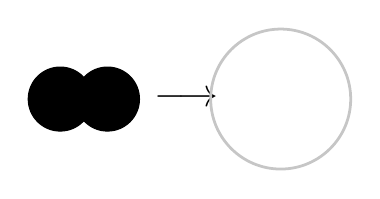
\begin{tikzpicture}
\filldraw[fill=black] (-0.3,0) circle (0.16in);
\filldraw[fill=black] (0.3,0) circle (0.16in);
\draw[line width=1.5pt] (-0.14,0) -- (0.14,0);
\node at (1.3,0) {\Large $\longrightarrow$};
\draw[line width=1pt, gray!45] (2.5,0) circle (0.35in);
\end{tikzpicture}
\end{center}

This gives a precise answer to Sproll 00's old question. The two dots, unbound, are two things, under an ordinary counting rule. The exact same two dots, once bound and collapsed under the merging rule, are one thing. Neither answer is more correct than the other; they describe different stages of the same construction, examined under different rules.

\begin{algorithmproc}{Building a Whole}
A collection of separate things becomes a treated-as-one whole only through two specific steps: first, the things must be bound together, and second, a Collapse rule must be applied that specifically treats bound things as a single unit. Skipping either step leaves you with separate parts, not a whole.
\end{algorithmproc}

\begin{practicenow}
Take two small separate objects (two coins, two buttons). Physically connect them somehow (tape, string, or simply holding them together in one hand). Describe, in your own words, the moment at which you would say they have become ``one thing you are holding'' rather than ``two things you are holding.''
\end{practicenow}

\begin{exercisebox}{Section 1.1}
\item Explain, using this workbook's vocabulary, why two unbound dots and the same two dots after binding and collapsing are both correct descriptions of ``how many things there are.''
\item Describe a real-life example of binding several separate items and then treating them, for some purpose, as one single unit.
\item Challenge: can something be bound but never collapsed into a whole? What would that situation look like?
\end{exercisebox}

\chapter{The Ghost of the Parts}

\section{A Whole That Remembers Its Pieces}

Here is the idea this workbook most wants to leave you with. When several bound parts are collapsed into a whole, the parts do not vanish, even though the whole is now, correctly, being treated as one thing. A model built from several toy blocks looks, from the outside, like a single finished model. But if you look closely, or take it apart, the individual blocks are still exactly there, and the model's own shape is a direct trace of how those specific blocks were placed and connected.

\begin{center}
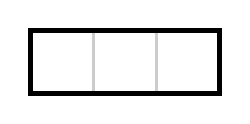
\begin{tikzpicture}
\draw[line width=1pt, gray!40] (-1.4,-0.4) rectangle (-0.6,0.4);
\draw[line width=1pt, gray!40] (-0.6,-0.4) rectangle (0.2,0.4);
\draw[line width=1pt, gray!40] (0.2,-0.4) rectangle (1,0.4);
\draw[line width=2pt] (-1.4,-0.4) rectangle (1,0.4);
\end{tikzpicture}
\end{center}

This is different from the melted candle from Sproll 05, where the original parts genuinely could not be recovered. A collapsed-into-one whole, in this curriculum's sense, keeps a kind of ghost outline of its construction available, even while being correctly treated as a single unit for most purposes.

\begin{algorithmproc}{Checking for a Ghost}
To check whether a whole still carries a trace of its parts, ask whether the construction could, even in principle, be taken apart or traced back to its original pieces. If yes, the whole has a past worth remembering, even while it is treated as one thing. If the parts are genuinely unrecoverable, something stronger than an ordinary collapse-into-whole has happened.
\end{algorithmproc}

\begin{trythis}
Build something small out of toy blocks, clay pieces, or even folded paper, using at least three separate pieces. Once finished, identify each original piece within the completed whole. Then, if you are willing, take it apart and confirm the pieces are exactly what you expected.
\end{trythis}

\begin{exercisebox}{Section 2.1}
\item Explain the difference between the toy-block model (a whole with a recoverable past) and the melted candles from Sproll 05 (a merge with no recoverable past).
\item Describe a real object in your life that is clearly ``one thing'' for most purposes but was built from separately identifiable parts you could, if you wanted, trace or take apart.
\item Challenge: can a whole lose its ghost of parts over time, becoming more like the melted candle, even if it did not start out that way? Give an example if you can.
\end{exercisebox}

\chapter{Building Bigger Wholes}

\section{Wholes Made of Wholes}

Nothing stops a whole, once collapsed, from later being bound to something else and collapsed again into a still bigger whole. Three toy blocks become one small tower. That tower, bound to two more small towers, becomes one larger structure. At every stage, the smaller wholes remain traceable inside the larger one, exactly as the individual blocks remained traceable inside each small tower.

\begin{summarybox}
A whole is built by binding separate parts and then collapsing them under a rule that treats bound things as one unit. Unlike a true merge, a collapsed whole ordinarily still carries a recoverable trace, a ghost, of the parts it was built from. This process can repeat: wholes can be bound and collapsed into still larger wholes, each level still tracing back to what it was built from.
\end{summarybox}

\begin{exercisebox}{Section 3.1}
\item Describe a real, multi-level example of wholes made from wholes (for example: letters into words, words into sentences, or rooms into a house).
\item At each level of your example, explain what the ``parts'' are and what the ``whole'' is.
\item Challenge: is it possible to tell, just by looking at a finished whole, how many levels of building went into it, without additional information? Explain your reasoning.
\end{exercisebox}

\chapter*{Looking Ahead}
\addcontentsline{toc}{chapter}{Looking Ahead}

All four primitive actions in this curriculum, Pop, Refuse, Bind, and Collapse, have now been introduced separately. The next workbook puts all four to work together, building one small, complete world from the ground up, to close out this first cycle of the Sproll Curriculum. That is the subject of Sproll 10: Four Moves Make a World.

\chapter*{For Parents and Teachers}
\addcontentsline{toc}{chapter}{For Parents and Teachers}

This workbook resolves Sproll 00's original ``many as one'' question precisely, using Bind and Collapse together: a whole is not simply declared to be one thing, it is constructed as one, through binding followed by a collapse under a rule that treats bound elements as a unit. The ``ghost of the parts'' idea anticipates a formal distinction this curriculum's technical companion material draws between a genuine merge (which discards the parts' separate identity entirely) and an ordinary collapse into a whole (which preserves a recoverable historical trace of its construction), though this workbook does not name that distinction formally.

\end{document}
